\section{15. Juni 2015}

\question{Elektronenkonfiguration von $B_2$ ($Z=5$)}
\label{q:31}

$B_2$ = $1\sigma_g^2 ~ 1\sigma_u^{*2} ~ 2\sigma_g^2 ~ 2\sigma_u^{*2} ~ 1\pi_u^2$ \\

\begin{figure}[H]
    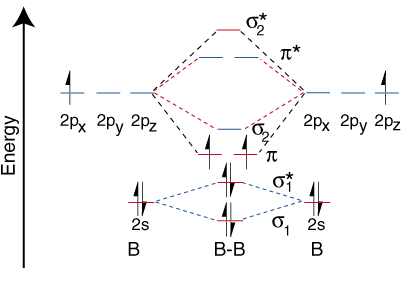
\includegraphics[width=0.8\linewidth]{resources/15-06-2015/b2.PNG}
    \caption{Elektronenkonfiguration von $B_2$}
\end{figure}

\question{Arten von Para-Diamagnetismus}
\label{q:32}

\question{Konzept von Bravais Wigner-Seitz Zelle}
\label{q:33}

Die Bravais Wigner-Seitz Zelle ist definiert als die Zelle im Raum, die jedem Gitterpunkt am nächsten 
liegt. Sie hat die folgenden Eigenschaften:
\begin{enumerate}
    \item Symmetrie: Die Zelle ist symmetrisch um den Gitterpunkt, von dem aus sie konstruiert wurde, sie weist alles Symmetrieoperationen, welche im gesamten Gitter vorkommen, auf. 
    \item Ein Gitterpunkt pro Zelle: Die Zelle enthält genau einen Gitterpunkt im Inneren der Zelle. Alle anderen Gitterpunkte des Gitters liegen auf den Seitenflächen der Zelle.
    \item Nächste Nachbarn: Die Zelle teilt den Raum so auf, dass jeder Gitterpunkt seinem nächstgelegenen Nachbarn am nächsten ist.
\end{enumerate}

Konstruktion:
\begin{figure}[H]
    \centering
    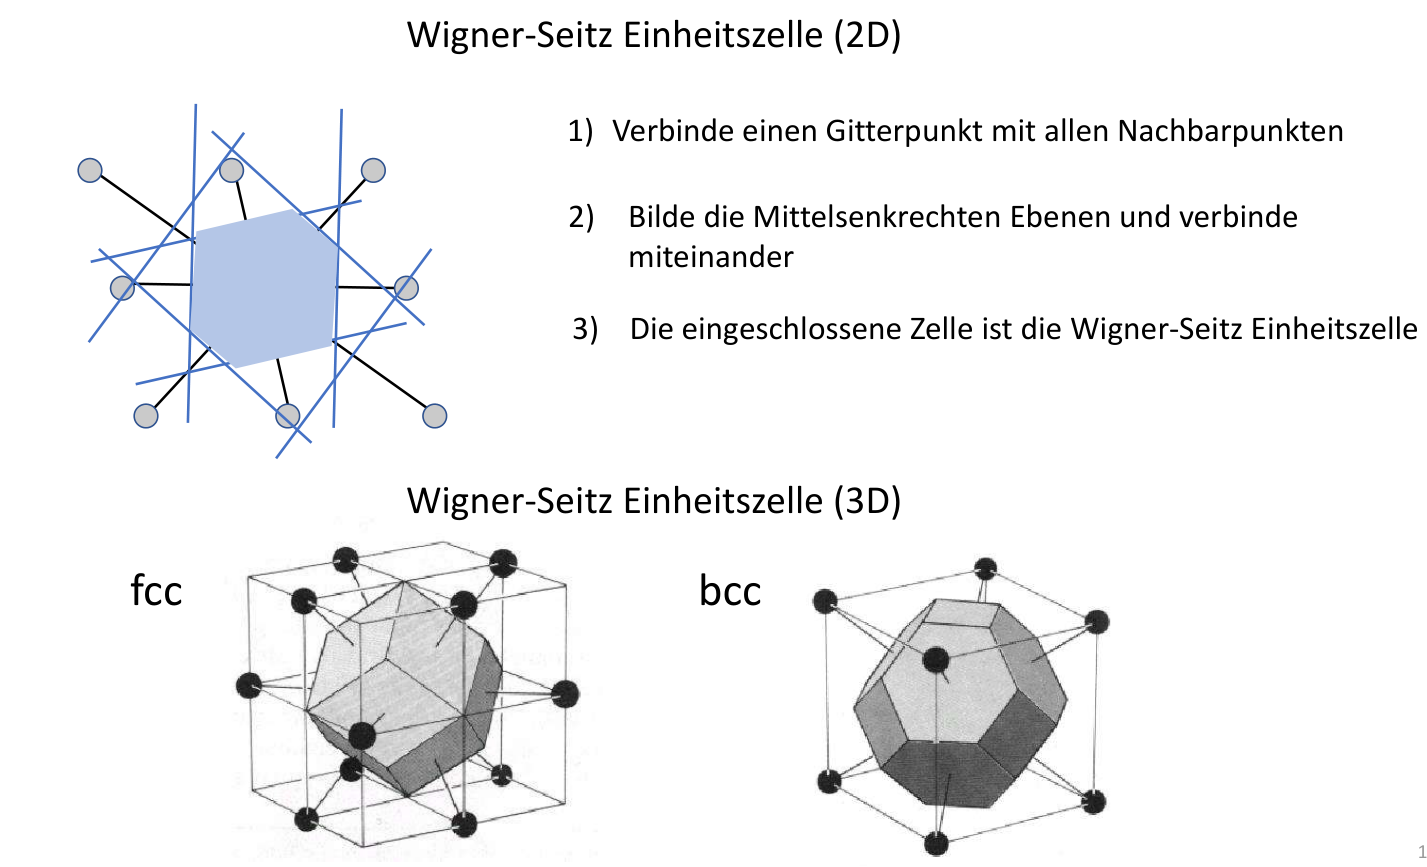
\includegraphics[width=0.8\linewidth]{resources/15-06-2015/q33.png}
    \caption{Konstruktion der Wigner-Seitz Zelle}
\end{figure}

\question{Sp sp2 sp3 Bindungen von mehratomigen Molekülen}
\label{q:34}

\question{Debye-Petit (oder so, irgendwas mit spezifischer Wärme von Elektronen)}
\label{q:35}

\question{Atom/Struktur Faktor}
\label{q:36}

\question{Zustandekommen von Energiebändern und Bandlöchern}
\label{q:37}

\question{Zusammenhang zwischen Gitterebene und Vektoren im reziproken Gitter}
\label{q:38}

Siehe \aqref{4}.

\question{Statische Abschirmung des Elektronengases}
\label{q:39}

\question{Einstein-Debye Unterschiede und falsche Annahmen}
\label{q:40}
\textbf{Einstein-Näherung} 
\begin{itemize}
    \item Annahme: alle Atome im Kristall schwingen mit der gleichen Frequenz $\omega$ = $\omega_E$, wobei $\omega_E$ die Frequenz der optischen Moden darstellt. 
    \item lässt sich nur auf optische Moden anwenden (nicht auf akkustische!)
    \item funktioniert gut bei hoher Dichte der optischen Phononen und liefert richtiges 
    Hochtermperaturlimit nach Dulong-Petit-Gesetz
    \item funktioniert schlecht bei tiefen Temperaturen und liefert ungenaues Limit für niedrige Temperaturen
    \item Falsche Annahme: akkustische Moden werden nicht berücksichtigt und alle harmonischen Oszillatoren im Festkörper würden mit einheitlicher Frequenz schwingen.
\end{itemize}

\textbf{Debye-Näherung} 
\begin{itemize}
    \item Annahme: 
        \begin{itemize}
            \item Vielzahl möglicher Frequenzen und Ausbreitungsgeschwindigkeit $v_i$ von Wellen/Phononen. 
            \item Lineare Dispersion $\omega_i=v_ik$ 
        \end{itemize}
    \item berücksichtigt nur akkustische Moden
    \item funktioniert gut bei niedrigen Temperaturen, da niederenergetische (akkustische) Phononen besser dargestellt sind 
    \item liefert korrektes Limit für hohe und tiefe Temperaturen
    \item Falsche Annahme: optische Phononen werden nicht berücksichtigt und Effekte nahe der Brillouinzonengrenze werden nicht richtig beschrieben
\end{itemize}

\begin{figure}[H]
 \centering
 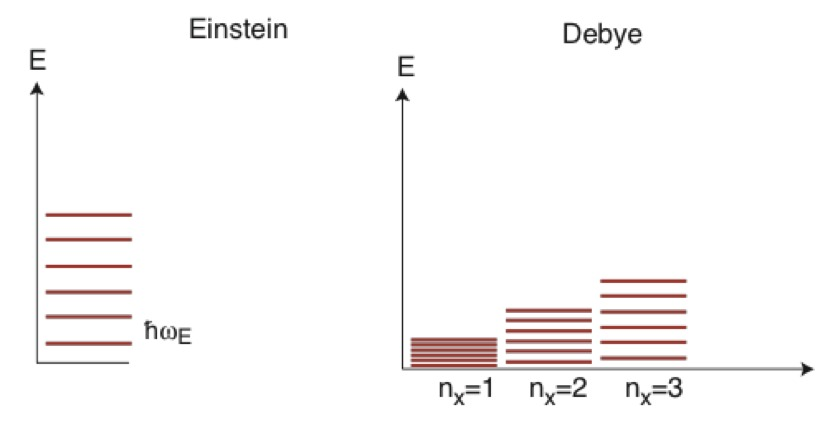
\includegraphics[width=0.6\textwidth]{resources/15-06-2015/Einstein_Debye.jpeg}
 \caption{Einstein- vs. Debye-Modell}
 %\label{}
\end{figure}
\newpage